\documentclass[tikz,border=10pt]{standalone}
\usepackage{tikz}

\begin{document}
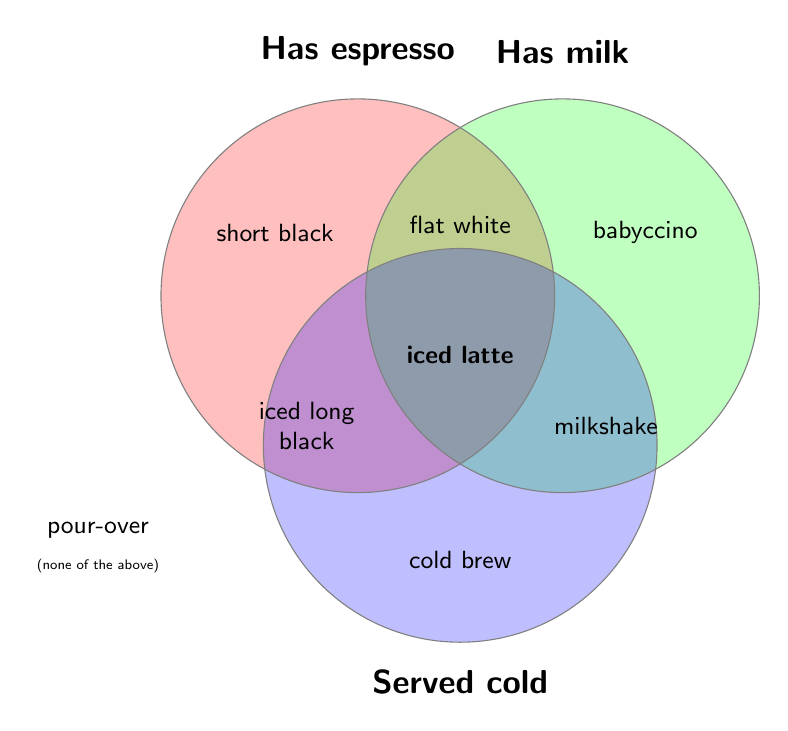
\begin{tikzpicture}[
    font=\sffamily\small,
  ]

  % --- Circles (drawn, so nothing is typeset inside them) ---------------
  \def\r{2.5cm}
  \begin{scope}
    \fill[red,   opacity=0.25] (-1.3, 0.9) circle (\r);
    \fill[green, opacity=0.25] ( 1.3, 0.9) circle (\r);
    \fill[blue,  opacity=0.25] ( 0.0,-1.0) circle (\r);
    \draw[gray] (-1.3, 0.9) circle (\r);
    \draw[gray] ( 1.3, 0.9) circle (\r);
    \draw[gray] ( 0.0,-1.0) circle (\r);
  \end{scope}

  % --- Region labels ---------------------------------------------------
  \node at (-2.35, 1.70) {short black};                 % espresso only
  \node at ( 2.35, 1.70) {babyccino};                   % milk only
  \node at ( 0.00,-2.45) {cold brew};                   % cold only
  \node at ( 0.00, 1.80) {flat white};                  % espresso + milk
  \node[align=center] at (-1.95,-0.75) {iced long\\black}; % espresso + cold
  \node at ( 1.85,-0.75) {milkshake};                   % milk + cold
  \node[font=\sffamily\small\bfseries] at ( 0.00, 0.15) {iced latte}; % all three
  \node[align=center] at (-4.60,-2.30) {pour-over\\[2pt]{\tiny (none of the above)}};

  % --- Set captions ----------------------------------------------------
  \node[font=\sffamily\large\bfseries] at (-1.3, 4.00) {Has espresso};
  \node[font=\sffamily\large\bfseries] at ( 1.3, 4.00) {Has milk};
  \node[font=\sffamily\large\bfseries] at ( 0.0,-4.00) {Served cold};

\end{tikzpicture}
\end{document}
